
\chapter{Il Progetto}

In questo capitolo si descrivono le caratteristiche principali del
sistema MatrixPro e dell'annesso Trakla2, evidenziando in particolar
modo le motivazioni che hanno portato quest'ultimo ad essere scelto
come fondamenta del progetto di tesi.


\section{\label{sec:MatrixPro-e-Trackla2}MatrixPro e Trakla2}


\subsection{Creare Animazioni con MatrixPro}

MatrixPro \cite{MatrixPro} è un software con licenza GPL2, ed è quindi
gratuito e open source. Il programma è stato creato per permettere
a studenti, ma soprattutto ad insegnanti, di creare velocemente animazioni
personalizzate su strutture dati pre-esistenti nel programma. L'applicazione
è molto utile come spiegano gli sviluppatori nell'articolo \cite{MatrixPro}
per rendere più coinvolgenti le lezioni universitarie, con presentazioni
animate precedentemente create dal docente, o persino create al volo
durante la spiegazione, per riuscire a rispondere con la dimostrazione
visiva a domande e dubbi degli studenti.

Tra i punti di forza di questo applicativo troviamo la semplicità
con cui possono essere utilizzate le strutture dati esistenti, ma
soprattutto la loro organizzazione. Le strutture sono suddivise in
due grandi gruppi: 
\begin{description}
\item [{{FDT}}] (Fundamental Data Types) che equivalgono alle strutture
primitive, alle quali non viene associata alcuna operazione o informazione
sematica riguardo al loro utilizzo. Tra queste troviamo liste, alberi,
grafi, array, chiavi. 
\item [{{CDT}}] (Conceptual Data Types) sono strutture che implementano
tipi di dato astratti e che necessitano di maggiori restrizioni. Possono
essere modificate solo tramite operazioni che ne alterano la struttura
secondo regole predefinite. Tra queste troviamo Alberi Binari di Ricerca,
Heap, Stack, e molte altre. 
\end{description}
Esistono inoltre altre strutture utilizzabili nella realizzazione
di un'animazione, che vengono chiamate {}``strutture utili'' (utilities),
e permettono di creare al volo un dati casuali o consentono altre
funzionalità allo stesso modo interessanti. Questa classificazione
in strutture primitive e avanzate aiuta l'utente a comprendere più
chiaramente la gerachia esistente tra i diversi sistemi, e a concentrarsi
maggiormente sulla parte concettuale del problema analizzato e non
sui dettagli implementativi.

In accordo con il principio sul controllo del flusso espresso dalla
guida per sviluppatori \cite{wikiAlgoViz}, le animazioni create sono
memorizzate all'interno del programma come una serie di passi, caratterizzati
da un particolare stato del sistema e di tutte le strutture coinvolte
nella visualizzione. All'utente è concessa la possibilità di esplorare
i vari stati tramite semplici comandi di Avanti - Indietro - Inizio
- Fine.

Una volta creata l'animazione desiderata, è possibile salvarla come
oggetto Java serializzabile, e potrà essere modificata nuovamente
in un secondo momento. Inoltre MatrixPro permette di esportare il
proprio lavoro in 3 formati:
\begin{description}
\item [{\LaTeX{}}] immagine in formato .tex che è possibile includere facilmente
nei documenti Latex;
\item [{SVG}] (Scalable Vector Graphics) l'esportazione in tale formato
permette di salvare un'animazione alla quale viene incluso anche un
pannello di controllo che permette di spostarsi avanti e indietro
in modo simile a come fa il software MatrixPro al suo interno;
\item [{PNG}] l'esportazione in formato PNG (Portable Network Graphics)
permette si creare una fotografia di un particolare momento dell'animazione
dell'algoritmo, che viene salvata in un file immagine PNG.
\end{description}

\subsection{Il sistema Trakla2}

Nella versione più recente del software, si trova all'interno del
pacchetto che viene fornito da MatrixPro una caratteristica molto
interessante, che è stata chiamata Trakla2. Questa parte del sistema
consiste in un insieme di {}``esercizi'', creati a partire dal sistema
MatrixPro, all'interno dei quali lo studente deve simulare il comportamento
di un particolare algoritmo interagendo con le strutture grafiche.
Si accede a questi esercizi tramite il menù Exercise nella barra dei
menu.

L'utente esegue i passi dell'algoritmo trascinando e rilasciando con
il mouse gli elementi delle strutture. I cambiamenti del sistema sono
automaticamente memorizzati ed è inoltre possibile tornare indietro
e modificare le azioni precedentemente eseguite.

Una volta conclusa la simulazione, lo studente ha a propria disposizione
tre interessanti funzionalità, a cui si accede sempre tramite il menu
Exercise.
\begin{description}
\item [{Grade}] la funzione Voto permette allo studente di sapere se ha
o meno eseguito una simulazione corretta. Nella maggior parte degli
esercizi la votazione viene espressa in numero di passi corretti nella
simulazione rispetto al numero dei passaggi totali. In altri esercizi,
in cui non ha senso parlare di successione di stati, la valutazione
viene esplicitamente fornita tramite un messaggio testuale come per
esempio {}``Esercizio corretto'' o {}``Esercizio non corretto'';
\item [{Model\_Answer}] nella finestra Model Answer si visualizza l'animazione
corretta della simulazione dell'algoritmo preso in considerazione.
Attraverso questa modalità lo studente che non ha ancora compreso
il meccanismo del problema in analisi può osservarne l'animazione
corretta. Questa caratteristica in sintesi è la visualizzazione che
gli altri software di AV forniscono agli utenti.
\item [{Compare}] (disponibile solo in alcuni esercizi) la funzione di
confronto può essere considerata la fusione tra le due precedenti.
Permette infatti all'utente di confrontare passo-passo il risultato
della propria animazione con quello fornito dal sistema.
\end{description}
Anche negli esercizi del sistema Trakla2 è possibile salvare ed esportare
l'animazione creata nei formati forniti da MatrixPro.

\begin{figure}
\centering
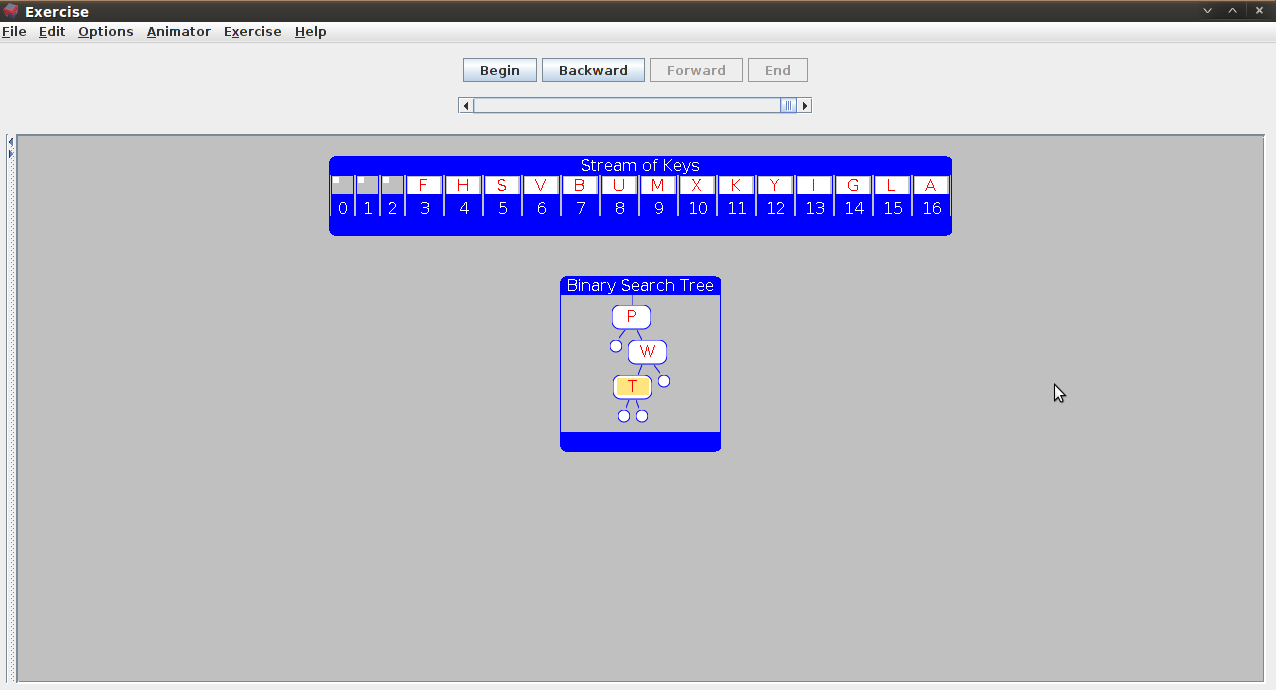
\includegraphics[scale=0.35]{images/trakla_screenshot.png}
\caption{Screenshot del sistema MatrixPro}
\end{figure}


\section{Motivazioni della scelta di MatrixPro}

In questa sezione si descrive il progetto che si intende realizzare
e le motivazioni che hanno portato alla scelta di MatrixPro come programma
base per la realizzazione dell'applicazione.


\subsection{Cosa si vuole realizzare}

Il progetto prevede la realizzazione di un software di visualizzazione
del comportamento degli algoritmi, destinato all'utilizzo da parte
degli studenti del corso di Algoritmi e Strutture Dati, con l'intento
di fornire un sussidio interattivo al libro di testo del corso.

Il software dovrà quindi coprire il più possibili gli argomenti trattati
nel programma del corso, e dovrà essere il più interattivo possibile
per coinvolgere al meglio gli studenti.


\subsection{Scelta del tool più adatto}

Per prima cosa è stata effettuata la ricerca di un applicativo pre-esistente
open source, dal quale partire e che sarà in seguito modificato, per
realizzare il nuovo software di visualizzazione di algoritmi.

Dopo una prima analisi degli strumenti trovati, descritti nella sezione
\ref{sec:Strumenti-Disponibili}, sono stati subito scartati tutti
i programmi che fornivano solo una presentazione animata degli algoritmi,
ovvero software come Animal. Questa scelta è stata fatta per garantire
l'interattività e il conseguente coinvolgimento degli studenti nell'utilizzo
dell'applicazione risultante.

La lista di software candidati si è quindi ristretta a 2 elementi:
JHAVÈ e MatrixPro.

Il primo è un'applicativo facilmente scaricabile ed eseguibile direttamente
dal browser, che si connette a particolari server all'interno dei
quali sono contenute animazioni di numerosi algoritmi. In aggiunta
alla visualizzazione dell'algoritmo, JHAVÈ fornisce allo studente
informazioni relative al problema, tra le quali per esempio lo pseudocodice
della soluzione, e interrompe l'animazione con domande inerenti alla
presentazione in corso dell'algoritmo.

MatrixPro, come spiegato in \ref{sec:MatrixPro-e-Trackla2}, concede
all'utente un livello maggiore di interattività, pur fornendo anche
un'animazione {}``normale'' di molti algoritmi come gli altri applicativi
disponibili. Per quest'ultimo motivo la scelta finale è ricaduta sul
software MatrixPro.
